% !TEX TS-program = XeLaTeX
% use the following command: 
% all document files must be coded in UTF-8
\documentclass{textolivre}
% for anonymous submission
%\documentclass[anonymous]{textolivre}
% to create HTML use 
%\documentclass{textolivre-html}
% See more information on the repository: https://github.com/leolca/textolivre

% Metadata
\begin{filecontents*}[overwrite]{article.xmpdata}
    \Title{Principales vertientes de los estudios de alfabetización en Brasil}
    \Author{Cícero da Silva \sep Adair Vieira Gonçalves}
    \Language{es}
    \Keywords{Estudios de alfabetización \sep Enseñanza-aprendizaje \sep Investigación \sep Brasil \sep Nuevos Estudios de Alfabetización}
    \Journaltitle{Texto Livre}
    \Journalnumber{1983-3652}
    \Volume{14}
    \Issue{1}
    \Firstpage{1}
    \Lastpage{16}
    \Doi{10.35699/1983-3652.2021.29164}

    \setRGBcolorprofile{sRGB_IEC61966-2-1_black_scaled.icc}
            {sRGB_IEC61966-2-1_black_scaled}
            {sRGB IEC61966 v2.1 with black scaling}
            {http://www.color.org}
\end{filecontents*}

% used to create dummy text for the template file
\definecolor{dark-gray}{gray}{0.35} % color used to display dummy texts
\usepackage{lipsum}
\SetLipsumParListSurrounders{\colorlet{oldcolor}{.}\color{dark-gray}}{\color{oldcolor}}

% used here only to provide the XeLaTeX and BibTeX logos
\usepackage{hologo}

% used in this example to provide source code environment
%\crefname{lstlisting}{lista}{listas}
%\Crefname{lstlisting}{Lista}{Listas}
%\usepackage{listings}
%\renewcommand\lstlistingname{Lista}
%\lstset{language=bash,
        breaklines=true,
        basicstyle=\linespread{1}\small\ttfamily,
        numbers=none,xleftmargin=0.5cm,
        frame=none,
        framexleftmargin=0.5em,
        framexrightmargin=0.5em,
        showstringspaces=false,
        upquote=true,
        commentstyle=\color{gray},
        literate=%
           {á}{{\'a}}1 {é}{{\'e}}1 {í}{{\'i}}1 {ó}{{\'o}}1 {ú}{{\'u}}1 
           {à}{{\`a}}1 {è}{{\`e}}1 {ì}{{\`i}}1 {ò}{{\`o}}1 {ù}{{\`u}}1
           {ã}{{\~a}}1 {ẽ}{{\~e}}1 {ĩ}{{\~i}}1 {õ}{{\~o}}1 {ũ}{{\~u}}1
           {â}{{\^a}}1 {ê}{{\^e}}1 {î}{{\^i}}1 {ô}{{\^o}}1 {û}{{\^u}}1
           {ä}{{\"a}}1 {ë}{{\"e}}1 {ï}{{\"i}}1 {ö}{{\"o}}1 {ü}{{\"u}}1
           {Á}{{\'A}}1 {É}{{\'E}}1 {Í}{{\'I}}1 {Ó}{{\'O}}1 {Ú}{{\'U}}1
           {À}{{\`A}}1 {È}{{\`E}}1 {Ì}{{\`I}}1 {Ò}{{\`O}}1 {Ù}{{\`U}}1
           {Ã}{{\~A}}1 {Ẽ}{{\~E}}1 {Ũ}{{\~u}}1 {Õ}{{\~O}}1 {Ũ}{{\~U}}1
           {Â}{{\^A}}1 {Ê}{{\^E}}1 {Î}{{\^I}}1 {Ô}{{\^O}}1 {Û}{{\^U}}1
           {Ä}{{\"A}}1 {Ë}{{\"E}}1 {Ï}{{\"I}}1 {Ö}{{\"O}}1 {Ü}{{\"U}}1
           {ç}{{\c{c}}}1 {Ç}{{\c{C}}}1
}


\journalname{Texto Livre: Linguagem e Tecnologia}
\thevolume{14}
\thenumber{1}
\theyear{2021}
\receiveddate{\DTMdisplaydate{2021}{1}{25}{-1}} % YYYY MM DD
\accepteddate{\DTMdisplaydate{2021}{3}{1}{-1}}
\publisheddate{\DTMdisplaydate{2021}{4}{5}{-1}}
% Corresponding author
\corrauthor{Cícero da Silva}
% DOI
\articledoi{10.35699/1983-3652.2021.29164}
% list of available sesscions in the journal: articles, dossier, reports, essays, reviews, interviews, editorial
\articlesessionname{Lingüística y Tecnología}
% Abbreviated author list for the running footer
\runningauthor{Silva y Gonçalves}
\editorname{Daniervelin Pereira}

\title{Principales vertientes de los estudios de alfabetización en Brasil}
\othertitle{Principais vertentes dos estudos do letramento no Brasil}
\othertitle{Main directions of literacy studies in Brazil}
% if there is a third language title, add here:
%\othertitle{Artikelvorlage zur Einreichung beim Texto Livre Journal}

%Não estão aparecendo todos os títulos!

\author[1]{Cícero da Silva \orcid{0000-0001-6071-6711} \thanks{Email: \url{cicolinas@yahoo.com.br}}}
\author[2]{Adair Vieira Gonçalves \orcid{0000-0003-4998-9692} \thanks{Email: \url{adairgoncalves@uol.com.br}}}

\affil[1]{Universidade Federal do Tocantins, Palmas, TO, Brasil.}
\affil[2]{Universidade Federal da Grande Dourados, Dourados, MS, Brasil.}

\addbibresource{article.bib}
% use biber instead of bibtex
% $ biber tl-article-template

% set language of the article
\setdefaultlanguage{spanish}
\setotherlanguage{portuguese}
\setotherlanguage{english}

% for spanish, use:
%\setdefaultlanguage{spanish}
%\gappto\captionsspanish{\renewcommand{\tablename}{Tabla}} % use 'Tabla' instead of 'Cuadro'

% for languages that use special fonts, you must provide the typeface that will be used
% \setotherlanguage{arabic}
% \newfontfamily\arabicfont[Script=Arabic]{Amiri}
% \newfontfamily\arabicfontsf[Script=Arabic]{Amiri}
% \newfontfamily\arabicfonttt[Script=Arabic]{Amiri}
%
% in the article, to add arabic text use: \textlang{arabic}{ ... }

\usepackage{tablefootnote}

\begin{document}
\maketitle

\begin{polyabstract}
\begin{abstract}
El objetivo de este artículo es contextualizar los estudios de alfabetización en Brasil, puntualizando las líneas de investigación y marcos teóricos principales. Esta exploración es de naturaleza bibliográfica, con un enfoque cualitativo-interpretativo. Primero, se plantean las referencias sobre los estudios de alfabetización y sus diferentes líneas, como la alfabetización académica, la escolar, la docente, la digital, la literaria y la científica. Luego, se realiza una consulta parametrizada en el sitio web del Directorio de Grupos de Investigación en Brasil, perteneciente al Consejo Nacional para el Desarrollo Científico y Tecnológico, donde se identifican las líneas y respectivos grupos investigativos vinculados a los estudios de alfabetización. Este levantamiento revela suficientes referencias sobre el tema, así como que las diversas perspectivas corroboran la trascendencia y las contribuciones de estas líneas investigativas, promovidas por el \textit{New London Group} y los Nuevos Estudios de Alfabetización.

\keywords{Estudios de alfabetización \sep Enseñanza-aprendizaje \sep Investigación \sep Brasil \sep Nuevos Estudios de Alfabetización}
\end{abstract}

\begin{portuguese}
\begin{abstract}
Neste artigo, objetiva-se contextualizar as vertentes dos estudos do letramento no Brasil, pontuando as principais linhas de investigação e referencial teórico. A pesquisa é de natureza bibliográfica, de abordagem qualitativo-interpretativista. Primeiramente, buscou-se na literatura referências que tratam de estudos do(s) letramento(s) e que se vinculam a diferentes linhas de pesquisa, como letramento acadêmico, letramento escolar, letramento do professor, letramento digital, letramento literário e letramento científico. Em seguida, realizou-se uma Consulta Parametrizada no sítio do Diretório dos Grupos de Pesquisa no Brasil do Conselho Nacional de Desenvolvimento Científico e Tecnológico para identificar as linhas de pesquisa e seus respectivos grupos de pesquisa vinculados aos estudos do(s) letramento(s) no Brasil. O estudo revelou que já existem bastantes referências acerca do tema no país e as perspectivas de investigação dos letramentos reforçam a importância e contribuições das pesquisas originárias no Grupo Nova Londres, alicerçadas pelos Novos Estudos do Letramento.

\keywords{Estudos do letramento \sep Ensino-aprendizagem \sep Pesquisa \sep Brasil \sep Novos Estudos do Letramento}
\end{abstract}
\end{portuguese}

\begin{english}
\begin{abstract}
In this paper, we contextualize the literacy studies in Brazil, providing the main lines of research and theoretical frameworks. The study is bibliographical with a qualitative-interpretative approach. First, we searched the literature for references related to literacy studies and the links to different research lines, such as academic literacy, school literacy, teacher’s literacy, digital literacy, literary literacy, and scientific literacy. Then, a parameterized consult was carried out on the website of the Directory of Research Groups in Brazil, from the National Council for Scientific and Technological Development, to identify the lines of research and their respective research groups related to literacy studies in Brazil. The study revealed that there are enough references on the subject and the prospects for literacy research reinforce the importance and contributions of the research originated in the New London Group and the New Literacy Studies.

\keywords{Literacy studies \sep Teaching-learning \sep Research \sep Brazil \sep New Literacy Studies}
\end{abstract}
\end{english}

% if there is another abstract, insert it here using the same scheme
\end{polyabstract}


\section{Palabras iniciales}\label{sec-intro}
El tema de las alfabetizaciones, por las dimensiones alcanzadas en el contexto académico brasileño de las últimas décadas, ha encauzado diferentes líneas de investigación, como la alfabetización académica, la escolar, la docente, la digital, la literaria, la científica, entre otras. En la misma medida, también ha aumentado el número de estudios sobre ellas, ya sea en forma de disertaciones, tesis, artículos o libros. De igual forma, las investigaciones desarrolladas se caracterizan por la existencia de diferentes perspectivas y metodologías, panorama que se presenta en este artículo.

Además de la lectura de trabajos de reconocidos autores en estudios de alfabetización en Brasil, realizamos en el año 2020 una consulta parametrizada en el sitio web del Directorio de Grupos de Investigación en Brasil (DGPB), del Consejo Nacional de Desarrollo Científico y Tecnológico (CNPq), para identificar las líneas de investigación (y sus respectivos grupos desarrolladores) con palabras claves tales como: alfabetización académica, alfabetización escolar, alfabetización docente, alfabetización digital, alfabetización literaria y alfabetización científica. Los resultados muestran que en ese año se registraron (en diferentes grupos de pesquisas de diversas instituciones de enseñanza e investigación de las regiones brasileñas), 13 líneas relacionadas con la alfabetización académica, 06 en alfabetización escolar, 03 en alfabetización docente, 20 en alfabetización digital, 18 en alfabetización literaria y 02 en alfabetización científica. Curiosamente, los números muestran que hay una cantidad notable de líneas que estudian la alfabetización digital y la literaria, mientras que en la docente solo se hallaron tres.

Los autores del artículo percibieron además que las líneas de estudio sobre alfabetización/es, tenían estrecha relación con sus respectivas investigaciones \cite{goncalves_nas_2011, goncalves_interacao_2013, silva_pedagogia_2018, silva_formacao_2019, silva_plano_2020, santos_letramento_2020}. También debe informarse que todas las tipologías de alfabetizaciones se imbrican y transforman. Por ello, nuestra opción de esbozarlas por separado es solo didáctica.

\section{Procedimientos metodológicos}\label{sec-metodologia}
Teniendo en cuenta el objetivo del estudio y la naturaleza de los datos, asumimos los procedimientos metodológicos de la investigación bibliográfica, con un enfoque cualitativo-interpretativo. Según \textcite[p. 9]{flick_introduco_2009}, “[...] la investigación cualitativa se basa en el texto y la escritura, desde las notas de campo hasta las transcripciones, pasando por las descripciones, y finalmente, por la interpretación de los resultados y la investigación en su conjunto.” Esta metodología contribuye en gran medida a la interpretación de los datos analizados, así como también permite investigar y reflexionar sobre el tema a partir de los datos recogidos de diversas formas.

Además, este artículo investigativo se desarrolla desde una perspectiva bibliográfica, o sea, a partir de “la revisión de la literatura sobre las principales teorías que orientan el trabajo científico. Este examen se conoce también como estudio bibliográfico o revisión de la literatura, que puede realizarse en libros, revistas, artículos de prensa, sitios de Internet, entre otras fuentes” \cite[p. 54]{pizzani_arte_2012}. Así, para contextualizar los estudios de alfabetización en Brasil, se realizó primero una pesquisa bibliográfica, componente esencial para situar las investigaciones desarrolladas sobre el tema. En otras palabras, identificamos y analizamos producciones académicas como libros, capítulos y artículos sobre el tópico en cuestión.

La revisión bibliográfica permite manejar definiciones del marco conceptual relacionado, apoyando los análisis a partir de los datos recopilados. Para ese propósito, primero se buscaron referencias relativas a los estudios de alfabetización/es vinculadas a las diferentes líneas de investigación, como la alfabetización académica, la escolar, la docente, la digital, la literaria y la científica.

Luego, se llevó a cabo una consulta parametrizada, el 17 de mayo de 2020, en el sitio web del Directorio de Grupos de Investigación en Brasil (DGPB), del Consejo Nacional de Desarrollo Científico y Tecnológico (CNPq) para identificar las líneas, sus respectivos grupos e instituciones de enseñanza e investigación vinculadas. La consulta empleó los siguientes parámetros o configuraciones de búsqueda: (1) Consultar “base actual”; (2) Censo: “ACTUAL”; (3) Término de búsqueda: “alfabetización digital”, por ejemplo, en “todas las palabras”; (4) Consulta por: “línea de investigación”; (5) Aplicar la búsqueda en los campos: “Nombre de la línea de investigación”; (6) Situación del grupo: “Certificado” o “No actualizado”. Los datos resultantes se recopilaron e ilustraron en tablas y gráficos.

\section{Alfabetización académica, escolar, docente, digital, literaria y científica}\label{sec-alfabetizacion}
Entendemos la alfabetización como el “estado o condición de quienes no solo saben leer y escribir, sino que cultivan y ejercitan las prácticas sociales que emplean la escritura” \cite[p. 47]{soares_escolarizacao_1999}. De esta definición inicial surgieron más tarde las diversas vertientes de los estudios de alfabetización/es en Brasil.

\subsection{Alfabetización académica}\label{sec-fmt-academica}
Partimos de la afirmación comprobada en varias investigaciones de que los géneros académicos no constituyen contenidos en las escuelas primarias y secundarias brasileñas. Así, es válido señalar que el desarrollo de la alfabetización académica podría realizarse, en cierto grado y dependiendo de las circunstancias, en la escuela secundaria, con la enseñanza de géneros del ámbito académico, teniendo en cuenta las relaciones intergenéricas \cite{correa_relacoes_2006}, como por ejemplo, la reseña, el resumen, el fichaje de referencias, el preproyecto de investigación, entre otros.

Al analizar las perspectivas teóricas y prácticas relacionadas con las alfabetizaciones académicas, \textcite{komesu_o_2014} indican que los estudios pioneros en lectura y escritura vinculados a este modelo de alfabetización se limitan a la educación superior, aunque el concepto también se puede aplicar desde los primeros años de la escuela primaria hasta la secundaria. Las prácticas de lectura y escritura, desde este punto de vista, son “prácticas sociales que varían según el contexto, la cultura y el género” \cite[p. 477]{komesu_o_2014}. A pesar de la existencia de variantes en dichas prácticas, entendemos que la alfabetización académica involucra principios pedagógicos, metodológicos y formativos, así como de interacción, similares en cualquier entorno educativo. Además, los géneros discursivos que median la lectura y la escritura en el aula, junto a sus modos de recepción, requieren del diálogo y el intercambio de conocimientos (locales o no) entre los actores sociales para la producción de significados.

No obstante la premisa defendida por \textcite{komesu_o_2014} y otros investigadores (no brasileños), de que la alfabetización académica abarca todos los niveles de educación (básico y superior); en la práctica, las investigaciones brasileñas que involucran los usos de la lectura, la escritura y sus tecnologías asociadas con la teoría de la alfabetización como práctica social en el entorno educativo (escuela o universidad), se vinculan a la llamada “alfabetización académica” o “alfabetización escolar”. En este último caso, se ajusta a las investigaciones desarrolladas en Educación Básica, como los estudios de \textcite{silva_pedagogia_2018, silva_plano_2020}.

Los supuestos teóricos que anclan las investigaciones y metodologías concernientes a la alfabetización académica, articulan las prácticas de lectura y escritura tanto de docentes como de estudiantes. En este sentido, la alfabetización académica estaría vinculada, de alguna manera, a actividades que implican géneros discursivos específicos de la academia. En diálogo con \textcite{lillis_student_2003}, \textcite[p. 37]{fiad_letramentos_2014}, se afirma que es necesario resaltar las relaciones dialógicas y de poder que se establecen entre “docente-alumno, docente-docente, alumno-alumno, docente-alumno-institución, profesor-alumno-comunidad científica, alumno-futura práctica docente, profesor-alumno-TDIC\footnote{Tecnologías Digitales de la Información y la Comunicación (TDIC).}, profesor-alumno-sociedad”, en las prácticas universitarias. Es decir, los géneros no deben estudiarse de forma aislada, sino vinculados a las relaciones discursivas \cite{lillis_student_2003} y al poder que establecen en las relaciones sociales.

Además, \textcite[p. 76]{zavala_quem_2010} considera que “[...] producir un texto académico es como cantar una canción con un coro detrás. [...] El académico no puede cantar solo porque las otras voces deben dar evidencia de lo que está cantando”. Comprender y aceptar esta condición significa que hay armonía (entre formador-aprendiz) en la construcción del conocimiento. Y los estudiantes deben estar conscientes de que en la producción de textos (no solo académicos) hay ida y vuelta, es decir, escritura, lectura, intervenciones y reescritura. Todo en sincronía entre alumno-docente.

Como demuestran otras investigaciones, la mayoría de las producciones textuales (individuales y/o colaborativas) representadas por los más variados géneros discursivos\footnote{Por ejemplo, los géneros redacción para el vestibular, resumen académico, reseña, informes de prácticas supervisadas, seminario, monografía y artículo científico. El vestibular es el examen de ingreso a las universidades brasileñas; es una prueba que evalúa los conocimientos adquiridos tanto en la escuela primaria como en la secundaria, siendo el principal medio de acceso a la educación universitaria de ese país.} orientados en el aula universitaria, ocupan un lugar destacado como objeto de investigación y enseñanza de la alfabetización académica en Brasil. Los trabajos de \textcite{marinho_escrita_2010, araujo_2013, fiad_letramentos_2014, santos_letramento_2020}, por ejemplo, son investigaciones afiliadas a este aspecto. En ellas, se diseñan rutas investigativas y análisis de datos con énfasis en la alfabetización ideológica \cite{street_literacy_1984, street_letramentos_2014}, caracterizándose la mayor parte de esos trabajos como etnográficos.

\subsection{Alfabetización escolar}\label{sec-escolar}
En Brasil, las investigaciones correspondientes a esta línea abordan temas tales como: usos y prácticas de lectura y escritura en la escuela (o fuera de ella); prácticas de lectura/escritura y gestión escolar del uso de espacios extracurriculares, como la biblioteca y la sala de informática; relación oralidad/escritura y alfabetización en producciones textuales; formación inicial, conocimientos docentes e implicaciones para la enseñanza de la lengua materna; metodologías y sus implicaciones en la enseñanza de la lectura/escritura orientada por géneros de otros ámbitos, como el periodismo, etc. Desde esta perspectiva, entendemos la alfabetización escolar como un

\begin{quote}
    [...] grupo de acciones individuales y colectivas, fundamentalmente vinculadas a aparatos institucionales de diversa índole, desde mobiliario y dispositivos de apoyo hasta reglamentos internos y programas de enseñanza, y no un conjunto de contenidos y metodologías que se van modificando o sustituyendo como consecuencia de las demandas oficiales y/o el acceso a las novedades académicas. \cite[p. 323]{signorini_letramento_2007}.
\end{quote}

\textcite{rojo_concepcoes_1995, rojo_letramento_2001, signorini_letramento_2007, bunzen_os_2010} representan la vertiente de la alfabetización escolar. \textcite{signorini_letramento_2007, rojo_letramento_2001}, principalmente, centran sus investigaciones en los enfrentamientos que implican las relaciones de los sujetos con las prácticas escolarizadas\footnote{Aunque no es el foco de este estudio, basándonos en \textcite{rojo_letramento_2001}, puede decirse que una práctica escolar se refiere a lo que es típico de la escuela, como la producción/lectura del género redacción para el vestibular. Una práctica escolarizada constituye lo introducido en el aula como objeto de didáctica, en este caso, puede ejemplificarse con la lectura y redacción del género artículo de opinión, propio del ámbito periodístico, pero que se utiliza frecuentemente en el contexto escolar.} de lectura y escritura.

La afirmación de la alfabetización escolar como el “modelo” en el que también se inscriben los procesos de enseñanza y aprendizaje de la lectura y la escritura en la escuela (o fuera de ella), se sustenta en la acción de los docentes y de grupo de actores (gestores, coordinadores escolares) involucrados en las prácticas educativas. Esta perspectiva incluye la enseñanza de las lenguas maternas como prácticas de alfabetización específica, pero “[...] que están en relación con la solidaridad y/o la confrontación con otras prácticas sociales dentro y fuera de la institución” \cite[p. 323]{signorini_letramento_2007}. En otros términos, significa que las prácticas de lectura y escritura en la escuela establecen nexos estrechos con contextos influyentes en la sociedad, como el ámbito académico y periodístico. Zavala plantea que

\begin{quote}
    [...] la alfabetización escolar es solo una forma de utilizar el lenguaje como parte de una práctica social que ha ganado legitimidad por razones ideológicas y que encaja en las relaciones de poder. Como consecuencia, los niños de orígenes minoritarios, que aprenden a usar el lenguaje de formas diferentes a como se enseña en la escuela, están en desventaja cuando deben adquirir el tipo de discurso expositivo y ensayístico que caracteriza la alfabetización escolar. \cite[p. 73]{zavala_quem_2010}.
\end{quote}

Aunque sea ampliamente aceptada y goce de mayor prestigio social, de la cita se deduce que la legitimación de la alfabetización escolar en el contexto educativo muchas veces no considera ni valora el conocimiento de los actores sociales pertenecientes a grupos minoritarios en el sistema educativo formal. Un niño que no domina la variante aceptada del idioma, por ejemplo, al producir un texto, podría enfrentar más dificultades que otros en la escritura. La minimización de tal choque depende directamente de las actitudes sensibles del docente durante el proceso de producción textual. Entre las principales acciones para revertir tal conflicto están el acompañamiento del alumno y su valoración, propiciándole contribuciones significativas para que desarrolle sus habilidades de lectura y escritura. Las investigaciones desarrolladas en las escuelas sobre la alfabetización escolar, por ejemplo, se refieren principalmente a las prácticas de lectura y escritura más cercanas a lo que \textcite{street_literacy_1984, street_letramentos_2014} denomina alfabetización autónoma.

\subsection{Alfabetización docente}\label{sec-docente}
Las investigaciones sobre la alfabetización docente guiadas por diversas perspectivas y metodologías han crecido significativamente en los últimos años y ocupan un lugar destacado, especialmente en el ámbito del desempeño profesional y la formación inicial y continua del profesorado en Brasil. Según \textcite[p. 21]{kleiman_projetos_2009}, podemos entender “[...] la alfabetización docente no como un mero instrumento para la realización del trabajo, sino como un aspecto constitutivo, identitario de su rol como formador de nuevos lectores y usuarios del lenguaje escrito, es decir, intrínsecamente ligado a su desempeño profesional”. Dentro de las investigaciones - ubicadas en contextos particulares -, la atención se centra en las prácticas de enseñanza y las identidades profesionales, la formación docente y la alfabetización, así como las políticas de formación profesoral y la alfabetización.

Esta vertiente, al tener amplias dimensiones y englobar el desempeño en el aula y la formación inicial y continua, tiene como principal objetivo crear condiciones para que el docente mejore sus (auto)representaciones sobre su capacidad profesional, así como la posibilidad de desarrollo autónomo de sus funciones en el entorno laboral \cite{kleiman_projetos_2009}. Las consecuencias de la actuación docente pueden en ocasiones reflejarse en las prácticas de enseñanza en las que este agente de alfabetización se despliega y participa en su espacio laboral, lo cual puede fortalecer las prácticas didáctico-pedagógicas del mismo.
La mayoría de las contribuciones sobre la alfabetización docente en Brasil provienen de investigaciones aplicadas a los estudios lingüísticos, como los trabajos de \textcite{kleiman_processos_2006, kleiman_projetos_2009, oliveira_variacao_2010, kleiman_estudos_2014}, entre otros. Estos presentan miradas reflexivas y un marco teórico que puede contribuir a la formación docente, la práctica profesional, la identidad del profesor como agente de alfabetización \cite{kleiman_processos_2006, kleiman_projetos_2009} y sus acciones en el ámbito laboral.

\subsection{Alfabetización digital}\label{sec-digital}
La interacción a través del lenguaje implica, principalmente en la contemporaneidad, prácticas de lectura y escritura mediadas por el uso de las llamadas Tecnologías Digitales de la Información y la Comunicación (TDICs); siendo prácticas bastantes comunes en la educación superior y de postgrado en diferentes modalidades de enseñanza (presencial y a distancia) e incluso en la educación básica. Esta realidad hace de las TDICs un importante medio facilitador de la interacción cultural y la representación social en las prácticas docentes y los eventos de alfabetización en contextos de formación. Todo lo cual ha posibilitado que la alfabetización digital figure como una línea de investigación relevante y de crecimiento potencial en el entorno académico brasileño.

El estudio de \textcite{araujo_letramento_2014}, además de discutir la trayectoria del (los) concepto(s) de alfabetización(es) digital(es) recurrente(s) en las décadas de 1970, 1980, 1990, hasta nuestros días, también presenta un panorama de las investigaciones desarrolladas en el área, puntualizando los más trascendentes sobre el tema y los respectivos métodos asumidos en esas pesquisas.

A lo largo de esos cinco decenios, los eventos de alfabetización que involucran prácticas de lectura y escritura vinculadas de alguna manera al uso de los TDICs y la enseñanza en el medio virtual, han recibido diferentes denominaciones: alfabetización visual, alfabetización tecnológica, alfabetización computacional, alfabetización de las TDIC, alfabetización informática y alfabetización electrónica \cite{araujo_letramento_2014}. Por tanto, el concepto de alfabetización digital está influenciado por todas estas designaciones. 

Basándose en \textcite{buzato_desafios_2007}, para quien la noción de alfabetización digital adquiere sentido debido al aspecto transcultural de Internet, \textcite[p. 301]{araujo_letramento_2014} entienden la alfabetización digital “[...] como una amalgama de diferentes tipos de alfabetizaciones que se entrelazan y apoyan mutuamente para que los sujetos puedan construirse y constituirse a través de sus relaciones sociales en entornos virtuales”. En otros términos, esta concepción contempla los usos sociales promovidos por los TDICs.

Entre las investigaciones referidas a la alfabetización digital relacionadas con la docencia en entornos virtuales, o el uso de los TDICs como soporte en el contexto educativo, podemos mencionar los trabajos de \textcite{coscarelli__letramento_2011, signorini_letramentos_2012, komesu_letramentos_2013, araujo_letramento_2014, vidotti_de_rezende_o_2016, ribeiro_tecnologia_2016}, entre otros. Los intereses investigativos en estos estudios recaen en el aprendizaje a través de la mediación tecnológica y presentan un estrecho vínculo con la alfabetización ideológica.

Dentro del mismo contexto brasileño es significativo destacar algunos textos recientes enfocados en la alfabetización digital, la docencia en el contexto de la pandemia COVID-19 y sus desafíos para profesores y estudiantes, como los de \textcite{almeida_letramento_2020, arruda__educacao_2020, carneiro_uso_2020, silva_letramento_2020}. Además de analizar las cuestiones inherentes a la alfabetización digital debido a las nuevas exigencias pedagógicas en la educación básica y superior resultantes de la pandemia, este conjunto de investigaciones también examina el acceso y la utilización de esos recursos tecnológicos, al mismo tiempo que destacan las experiencias y prácticas pedagógicas mediadas por TDICs en la educación brasileña.

\subsection{Alfabetización literaria}\label{sec-literaria}
La discusión sobre aspectos teóricos y metodológicos relacionados con la alfabetización literaria en Brasil constituye, en la actualidad, un tema que no puede pasar desapercibido en investigaciones académicas como este artículo, dada las evidencias de las prácticas de lectura y escritura en diferentes ámbitos sociales que involucran textos literarios. En este sentido, la alfabetización literaria designa una parte de esta como un todo, caracterizándose por la inserción de actores sociales en el mundo de la escritura, a través de las prácticas de recepción/producción de diferentes tipos de textos escritos que circulan en la sociedad \cite{paulino_letramento_2001}. 

En su libro, \textcite{cosson_letramento_2009} se centra en el proceso de alfabetización inherente a los textos literarios, al mismo tiempo, propone la formación de una comunidad de lectores que trascienda los límites del aula y la escuela. De esto se colige que, el proceso de alfabetización literaria es diferente al de la lectura literaria por fruición; es decir, esta depende de aquella. Por tanto, cuando empleamos la literatura en el aula con fines didácticos

\begin{quote}
    [...] debemos entender que la alfabetización literaria es una práctica social y, como tal, una responsabilidad de la escuela. La pregunta que hay que afrontar no es si la escuela debería o no escolarizar la literatura, como advierte Magda Soares, sino cómo llevar a cabo esta escolarización sin caracterizarla mal, sin transformarla en un simulacro de sí mismo que niega más que confirma su poder humanizador. \cite[p. 23]{cosson_letramento_2009}. 
\end{quote}

Desde el punto de vista de la alfabetización literaria, no se puede exigir al alumno que solo lea una determinada obra y, al final, realice una prueba o entregue fichas de lectura, ya que la lectura se desarrolla sobre la base de los mecanismos propuestos por la escuela para el dominio de la lectura literaria. \textcite{cosson_letramento_2009}, al discutir lo que denomina escolarización de la lectura literaria en la enseñanza, sugiere alternativas que apuntan a minimizar el tratamiento escolar negativo de la literatura, señalando ciertos conceptos erróneos y algunas alternativas accesibles a los maestros. 

Entre las principales investigaciones centradas en la alfabetización literaria, referentes a las prácticas de lectura y escritura escolares u otros ámbitos sociales que involucren textos literarios, destacamos los trabajos de \textcite{lajolo_leitura_1991, soares_escolarizacao_1999, paulino_letramento_2001, cosson_letramento_2009}, entre otros. Estos han proporcionado contribuciones importantes al desarrollo investigativo de la alfabetización literaria en Brasil. 

\subsection{Alfabetización científica}\label{sec-cientifica}
Tal como se ha expuesto, los diferentes aspectos de los estudios de alfabetización brasileños contemporáneos, están alineados con los más variados usos del lenguaje en la lectura, la escritura y sus tecnologías en las prácticas sociales. En el centro de estas prácticas de uso del lenguaje, emerge también la llamada alfabetización científica como objeto investigativo notable \cite{santos_educacao_2007, cunha_alfabetizacao_2017}.   

Desde esta perspectiva, la problematización de la enseñanza del lenguaje científico en el aula, así como sus implicaciones para la cultura científica de la sociedad, son puntos que requieren de una reflexión detenida. \textcite[p. 479]{santos_educacao_2007} señala que

\begin{quote}
    [...] en la tradición escolar, la educación científica se ha considerado en el sentido del dominio del lenguaje científico, mientras que la alfabetización científica, en el sentido del uso de la práctica social, parece ser un mito lejano a la práctica en el aula. Al usar el término alfabetización, buscamos enfatizar la función social de la educación científica en oposición al significado restringido de \textit{alfabetización escolar}. 
\end{quote}

Según la cita, se entiende que la \textit{alfabetización}\footnote{Usamos aquí el término en el sentido de los conocimientos básicos de la lecto-escritura.} sería el proceso más elemental para dominar el lenguaje científico. A su vez, la alfabetización científica requiere tanto del dominio del lenguaje científico (en la escritura) como de la práctica social, lográndose así la educación científica deseada en sus diferentes grados, en los procesos cognitivos y dominios de alto nivel \cite{santos_educacao_2007}. En otros términos, la alfabetización científica es “el proceso mediante el cual los estudiantes acceden al conocimiento científico y su producción, mediado por la escritura, de manera que posibilite una visión e intervención consciente y crítica en el mundo real” \cite[p. 7]{silva_ciencia_2018}. De tal modo, la alfabetización científica ofrece la capacidad de emplear el lenguaje para transitar con fluidez por los diversos acontecimientos de la vida cotidiana vinculados, de disímiles maneras, a saberes científicos determinados.

La educación científica contribuye a la comprensión del mundo que nos rodea y resulta fundamental para la constitución del pensamiento crítico del alumnado en el proceso de formación, preparándolos como actores sociales capaces de visualizar la importancia de la alfabetización científica en el desarrollo de investigaciones sobre diversas ciencias u otras áreas.   

Por tales razones, este tipo de alfabetización ha ocupado un espacio destacado en la investigación brasileña relacionada con las diferentes áreas de la educación científica: las cuales sitúan referencias, reflexionan sobre el currículo, la filosofía, la política educativa, la escritura académica o la formación de profesores, en un intento de analizar el papel social de la educación científica en la formación de los ciudadanos \cite{santos_educacao_2007}. La mayor parte de las contribuciones sobre esta alfabetización provienen de investigaciones del área de las ciencias y los estudios del lenguaje, tales como los trabajos de \textcite{santos_educacao_2007, motta-roth_letramento_2011, cunha_alfabetizacao_2017, silva_ciencia_2018}, entre otros.

\subsection{Discusión}\label{sec-discusion}
Para ilustrar los resultados de la consulta parametrizada realizada en el Directorio de Grupos de Investigación en Brasil (DGPB), del \textcite{consejo_nacional_de_desarrollo_cientifico_y_tecnologico__cnpq_directorio_nodate}\footnote{Para más detalles, consúltese el sitio web del Directorio de Grupos de Investigación de Brasil/CNPq en \url{http://dgp.cnpq.br/dgp/faces/consulta/consulta_parametrizada.jsf}.}, y con el fin de identificar las líneas de investigación previamente caracterizadas, se diseña el \Cref{tbl01}.

\begin{table}[htpb]
\caption{Distribución de las líneas de investigación sobre alfabetizaciones en el DGPB/CNPq.}
\label{tbl01}
\begin{tabular}{llll}
\toprule
\textbf{Línea de investigación}    & \textbf{Cantidad} & \textbf{\%}    & \textbf{Instituición\tablefootnote{Leyenda de las siglas de instituciones de enseñanza e investigación brasileñas: IFBA - Instituto Federal da Bahia; IFCE - Instituto Federal do Ceará; IF-Farroupilha - Instituto Federal Farroupilha; IFRN - Instituto Federal do Rio Grande do Norte; IFRS - Instituto Federal do Rio Grande do Sul; IFSC - Instituto Federal de Santa Catarina; PUC/PR - Pontifícia Universidade Católica do Paraná; UEM - Universidade Estadual de Maringá; UEMA - Universidade Estadual do Maranhão; UEMASUL - Universidade Estadual da Região Tocantina do Maranhão; UERGS - Universidade Estadual do Rio Grande do Sul; UESPI - Universidade Estadual do Piauí; UERJ - Universidade do Estado do Rio de Janeiro; UESB - Universidade Estadual do Sudoeste da Bahia; UESC - Universidade Estadual de Santa Cruz; UFAL - Universidade Federal de Alagoas; UFBA - Universidade Federal da Bahia; UFERSA - Universidade Federal Rural do Semi-Árido; UEMG - Universidade do Estado de Minas Gerais; UFMG - Universidade Federal de Minas Gerais; UFPA - Universidade Federal do Pará; UFPB - Universidade Federal da Paraíba; UFPE - Universidade Federal de Pernambuco; UFPR - Universidade Federal do Paraná; UFRB - Universidade Federal do Recôncavo da Bahia; UFRN - Universidade Federal do Rio Grande do Norte; UFRPE - Universidade Federal Rural de Pernambuco; UFRR - Universidade Federal de Roraima; UFSCar - Universidade Federal de São Carlos; UFSJ - Universidade Federal de São João Del-Rei; UFSM - Universidade Federal de Santa Maria; UFT - Universidade Federal do Tocantins; UFTM - Universidade Federal do Triângulo Mineiro; UNEB - Universidade do Estado da Bahia; UNESP - Universidade Estadual Paulista Júlio de Mesquita; UNICAMP - Universidade Estadual de Campinas; UNIOESTE - Universidade Estadual do Oeste do Paraná; UNIPAMPA - Universidade Federal do Pampa; UNIR - Universidade Federal de Rondônia; UNITAU - Universidade de Taubaté; UNIVILLE - Universidade da Região de Joinville; USP - Universidade de São Paulo; UTFPR - Universidade Tecnológica Federal do Paraná.}}            \\
\midrule
L1. Alfabetización académica &
  13 &
  21\% &
  \begin{tabular}[c]{@{}l@{}}IFCE, UNIVILLE, UEM, UFERSA, IFRS, \\ UFT, PUC/PR, UTFPR, UFMG, IFBA, \\ UFRB, UFPR, UFSJ\end{tabular} \\
\midrule
L2. Alfabetización escolar         & 6                 & 10\%           & USP, UERJ, UEMASUL, UFMG, UFSCar \\
\midrule
L3. Alfabetización docente         & 3                 & 5\%            & UFPE, UNITAU, UNICAMP            \\
\midrule
L4. Alfabetización digital &
  20 &
  32\% &
  \begin{tabular}[c]{@{}l@{}}UEMA, UFPR, UFRPE, UEMG, UFMG, \\ UFRN, UNIPAMPA, UNIVILLE, IFSC, \\ UFERSA, UNITAU, UFSCar, UFSM, \\ UESB, UFBA, UFPB, UTFPR, UNEB, \\ UNESP\end{tabular} \\
\midrule
L5. Alfabetización literaria &
  18 &
  29\% &
  \begin{tabular}[c]{@{}l@{}}UESC, UFRR, UFAL, UFMG, UFTM, UFT, \\ UNIVILLE, UFPE, UFPA, IFRN, UNIR, \\ UNITAU, IF-Farroupilha, UERGS, \\ UNIOESTE\end{tabular} \\
\midrule
L6. Alfabetización científica      & 2                 & 3\%            & UESPI, IFSC                      \\
\multicolumn{1}{c}{\textbf{Total}} & \textbf{62}       & \textbf{100\%} &  \\
\bottomrule
\end{tabular}
\source{datos de la investigación (2020).}
\end{table}

%não está aparecendo a nota de rodapé 6, inserida na tabela. Deve ser pq é longa

Los datos muestran los siguientes números de líneas de investigación sobre alfabetizaciones registradas en el DGPB/CNPq: 13 en \textit{L1. Alfabetización académica}; 06 en \textit{L2. Alfabetización escolar}; 03 en \textit{L3. Alfabetización docente}; 20 en \textit{L4. Alfabetización digital}; 18 en \textit{L5. Alfabetización literaria}; y 02 en \textit{L6. Alfabetización científica}. En total, se identificaron 62 líneas, procedentes de 43 instituciones de enseñanza e investigación brasileñas. 

\begin{figure}[htbp]
 \centering
 
\includegraphics[width=0.85\textwidth]{Fig01.png}
 \caption{Participación de L1, L2, L3, L4, L5 y L6 en el universo de las 62 líneas de investigación.}
 \label{fig01}
 \source{datos de la investigación (2020).}
\end{figure}

Considerando las 62 líneas sobre alfabetizaciones identificadas en el DGPB/CNPq, se derivan los porcentajes siguientes: L1, 21\%; L2, 10\%; L3, 5\%; L4, 32\%; L5, 29\%; y L6, 3\%. Estas cifras ilustradas en el \Cref{fig01}, sugieren que L4 y L5 son predominantes, con 32\% y 29\%, respectivamente. En el caso de L4, tal magnitud se explica por el hecho de que el empleo de las TDICs en la vida cotidiana y en los entornos educativos actuales es muy común. Evidentemente, el uso de las tecnologías digitales que soportan los diferentes medios de comunicación (escritos y orales) en las prácticas sociales genera demandas, especialmente de enseñanza, todo lo cual está directamente vinculado a la alfabetización digital.  

Debe hacerse notar también que, si bien L3 es fundamental para el desarrollo de la educación, solo tiene el 5\% de los registros en el DGPB/CNPq. A continuación, presentamos el \Cref{fig02} donde se muestra la distribución de las líneas investigativas sobre alfabetizaciones en las diferentes regiones brasileñas.

\begin{figure}[htbp]
 \centering
 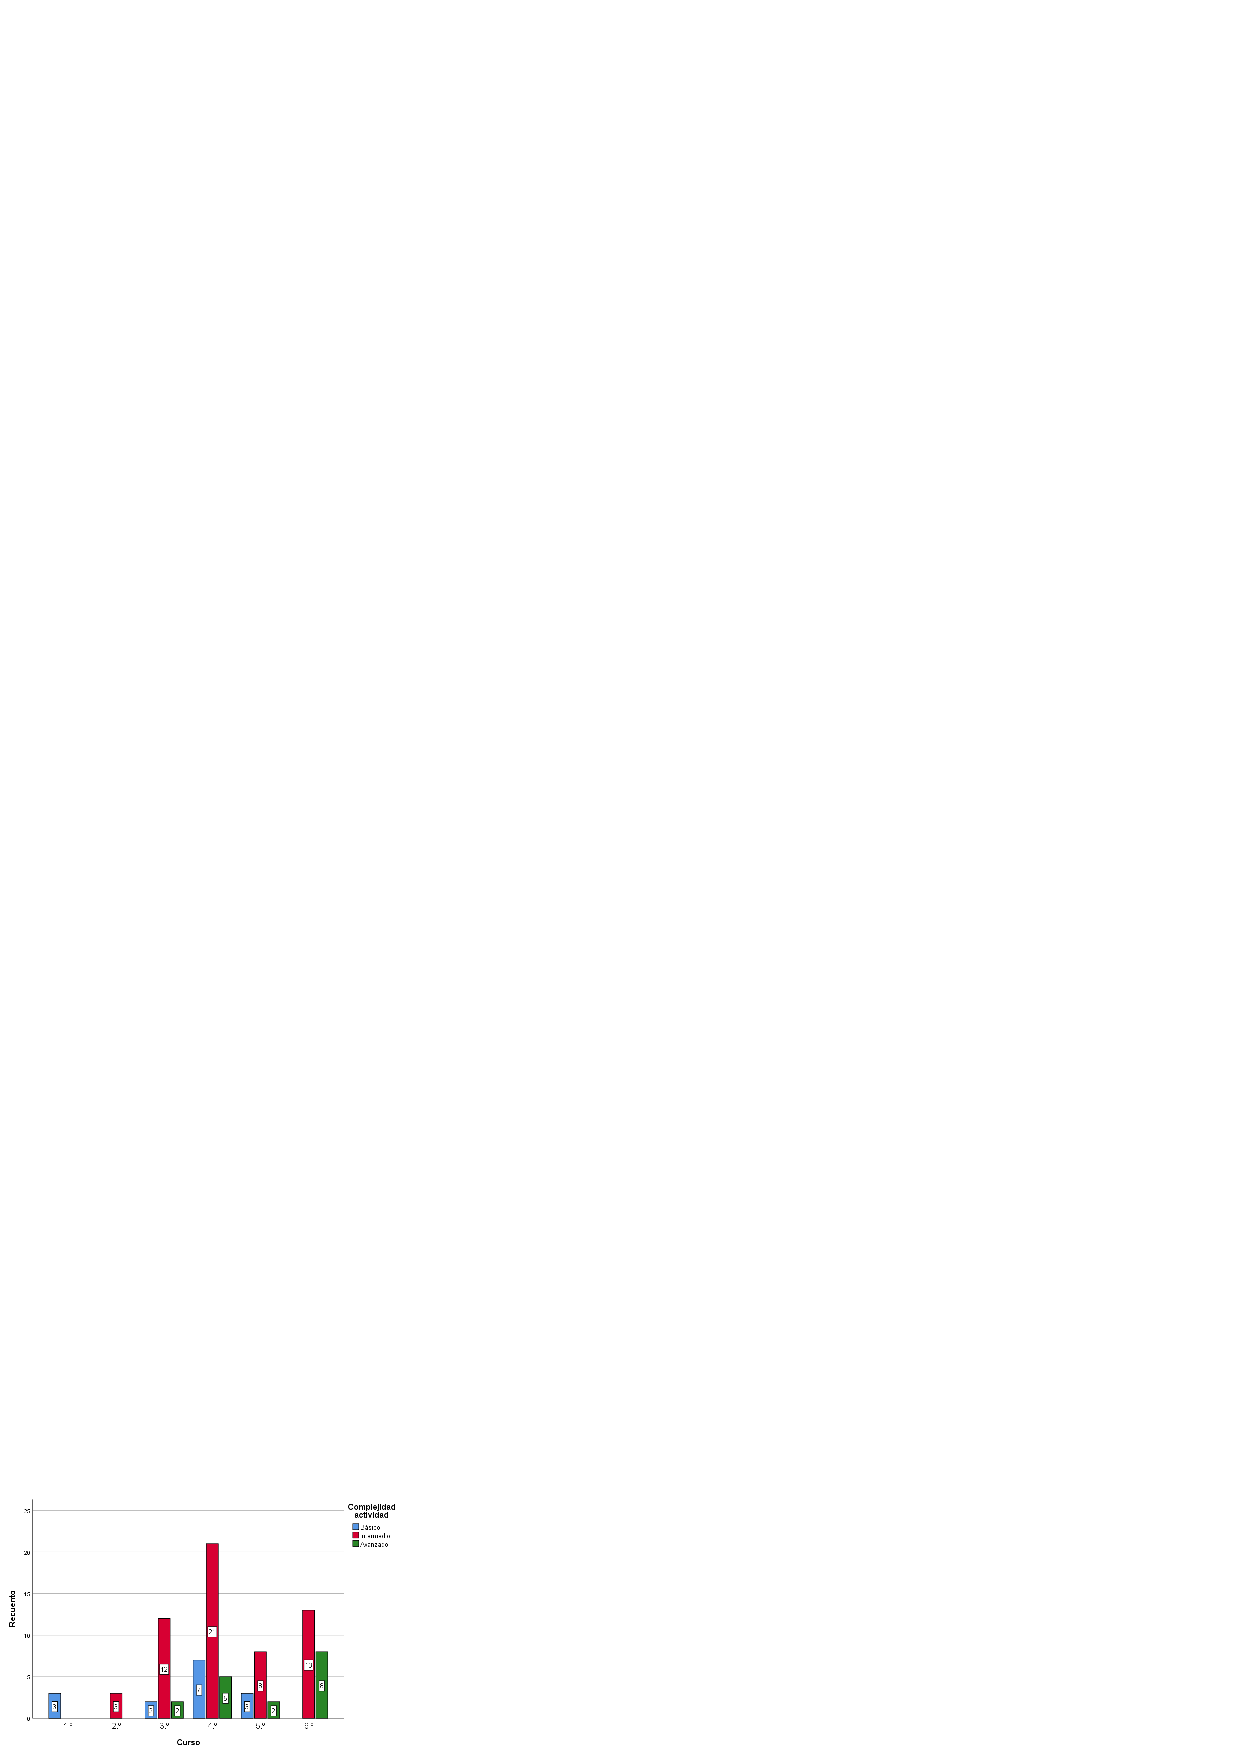
\includegraphics[width=0.85\textwidth]{Fig02.png}
 \caption{Distribución de las líneas de investigación sobre alfabetizaciones por regiones geográficas en Brasil, según el DGPB/CNPq.}
 \label{fig02}
 \source{datos de la investigación (2020).}
\end{figure}

Como se ilustró en el \Cref{tbl01}, las 62 líneas sobre alfabetizaciones (L1, L2, L3, L4, L5 y L6) están vinculadas a grupos investigativos de 43 instituciones educativas y de pesquisa brasileñas. En la secuencia, basada en los datos del \Cref{tbl01} y de la \Cref{fig02}, nos acercaremos a los respectivos números de líneas distribuidas en las cinco grandes regiones geográficas de Brasil.

\textit{L1. Alfabetización académica}: \Cref{tbl01} muestra que L1 tiene un total de 13 líneas registradas en los diferentes grupos investigativos del DGPB/CNPq. Están vinculadas a trece instituciones a saber: IFCE, UNIVILLE, UEM, UFERSA, IFRS, UFT, PUC / PR, UTFPR, UFMG, IFBA, UFRB, UFPR y UFSJ. Considerando la distribución geográfica, \Cref{fig02} revela que L1 tiene una línea en el Norte, seis en el Sur, dos en el Sureste y cuatro en el Noreste.

\textit{L2. Alfabetización escolar}: cuenta con seis líneas registradas en el DGPB/CNPq. La investigación muestra que L2 está vinculada a cinco instituciones: USP, UERJ, UEMASUL, UFMG y UFSCar. Debe señalarse que la UFMG tiene dos registros en L2, procedentes de dos grupos de investigación diferentes. Según la \Cref{fig02}, L2 está presente solo en dos regiones brasileñas, posee una línea en el Noreste y cinco en el Sureste. 

\textit{L3. Alfabetización docente}: se encontraron tres registros de L3 vinculados a tres grupos de investigativos de tres instituciones diferentes: UFPE, UNITAU y UNICAMP. La \Cref{fig02} revela que provienen de dos regiones: una línea en el Noreste y dos en el Sureste.

\textit{L4. Alfabetización digital}: de esta tipología se encontraron 20 registros en el DGPB/CNPq. Como se planteó anteriormente, es la de mayor cantidad de registros hallados, procedentes de 19 instituciones: IFSC, UNIVILLE, UNITAU, UNEB, UEMG, UEMA, UESB, UNESP, UFBA, UFPB, UFMG, UFSM, UFSCar, UNIPAMPA, UFPR, UFRN, UFRPE, UFERSA y UTFPR. Cabe mencionar que la UFERSA cuenta con dos registros en L4, vinculados a dos grupos de investigación diferentes. En cuanto a la distribución geográfica, tiene seis registros en el Sur, cinco en el Sureste y nueve en el Noreste.

\textit{L5. Alfabetización literaria}: la investigación indica que L5 alcanzó 18 registros en el DGPB/CNPq, por lo que es la segunda línea de mayor incidencia cuantitativa. Estos registros pertenecen a 15 instituciones: UESC, UFRR, UFAL, UFMG, UFTM, UFT, UNIVILLE, UFPE, UFPA, IFRN, UNIR, UNITAU, IF-Farroupilha, UERGS y UNIOESTE. Debe resaltarse que la UNIR tiene tres registros y la UFPA dos, provenientes de diferentes grupos de investigación.  Esta línea está distribuida con siete registros en el Norte, cuatro en el Sur, tres en el Sureste y cuatro en el Noreste. 

\textit{L6. Alfabetización científica}: según los resultados del \Cref{tbl01}, L6 posee dos registros afines a dos grupos de investigación de la UESPI y la IFSC. Aunque esta línea tiene un número razonable de artículos publicados, posee poca presencia en los grupos de investigación brasileños: tiene un registro en el Sur y otro en el Noreste. 

Debe indicarse que no se encontró ninguna línea de investigación sobre alfabetizaciones (L1, L2, L3, L4, L5 y L6) en instituciones de enseñanza e investigación de la región Centro Oeste brasileña. Aunque esto no significa la inexistencia de grupos de pesquisa sobre ellas en esa región. Sin embargo, la presencia de cualquiera de estas líneas en los grupos investigativos es importante para ampliar y fortalecer los estudios de alfabetización/es a nivel nacional. Otro hallazgo notable es que, entre las cinco regiones, solo la Nordeste tiene registros de las seis líneas investigadas en el DGPB/CNPq.

\section{Conclusiones}\label{sec-conclusiones}
Las perspectivas investigativas sobre las alfabetizaciones (académica, escolar, docente, digital, literaria y científica), corroboran la relevancia y aportes del \textit{New London Group} y los Nuevos Estudios de Alfabetización para el contexto brasileño. En esa dirección, el trabajo de \textcite{terra_letramento_2013} se propone contribuir a una mejor comprensión de las alfabetizaciones, discutiendo las formas conque ese fenómeno se ha abordado en conexión con los usos de la escritura en entornos educativos, en función de su naturaleza, y contexto cultural, así como sus consecuencias para la sociedad y las personas. Después de problematizar algunas cuestiones sobre la alfabetización, \textcite[p. 29]{terra_letramento_2013} concluye que los Nuevos Estudios de Alfabetización “son un camino fructífero para la (re)definición de una alfabetización escolar capaz de brindar a los estudiantes la oportunidad de aplicar en sus vidas cotidianas lo que aprenden en la escuela”. En otros términos, la alfabetización proporcionada en las actividades escolares debe, de alguna manera, estar vinculada a la realidad habitual de los estudiantes.

Además, la investigación sobre el uso de las Tecnologías Digitales de la Información y la Comunicación en las escuelas brasileñas realizada por el CGI.br en 2019, demuestra un uso intensivo de las tecnologías entre los estudiantes en actividades generales, como el acceso a las redes sociales (81\%), mensajería por aplicaciones (89\%) y el consumo de videos, programas, películas y series en Internet (94\%) \cite{comite_gestor_da_internet_no_brasil_resumo_2019}. Sin embargo, también revela que el empleo de estos recursos en actividades escolares, especialmente a través de la educación a distancia, aún no formaba parte del día a día de la mayoría de los alumnos. 

De igual forma, el 59\% de los profesores de las escuelas públicas urbanas brasileñas aludieron a la falta de un curso específico sobre usos de las tecnologías en actividades de enseñanza y aprendizaje. Estas dificultades fueron referidas también por el 29\% de los docentes de escuelas privadas. Aunque estos números corresponden a la educación básica, de cierta manera se reflejarán también en la educación superior, además de mostrar que no solo quienes laboran en el sistema escolar público enfrentan dificultades para aplicar las TDICs en sus prácticas didáctico-pedagógicas. Todo lo cual se traduce en demandas referentes a las alfabetizaciones digitales en el país.  

Asimismo, sumado a la falta de dominio o conocimiento de las tecnologías de enseñanza por parte de algunos docentes y alumnos, no debe olvidarse que una parte de estos últimos no tiene acceso a Internet de banda ancha, 3G/4G, o su calidad no es buena; como lo demuestran los datos sobre el acceso a Internet en el hogar y la enseñanza a distancia durante la pandemia de COVID-19 en Brasil \cite{nascimento_acesso_2020}. La alfabetización digital también está condicionada por estos hechos. Por ende, estas observaciones refuerzan la necesidad de desarrollar investigaciones centradas en la enseñanza, la alfabetización digital y el uso de las TDICs. Como demuestran los datos develados en este artículo, el gran número (20) de líneas de investigación en alfabetización digital registradas en el DGPB/CNPq, parecen ir en esta dirección.

\section{Agradecimientos}\label{sec-agradecimentos}
Los autores agradecen al Doctor Ivan Gabriel Grajales Melian por la lectura y revisión en lengua española de este documento.

\printbibliography\label{sec-bib}

\end{document}
